\section{Introduction}
\label{cha:introduction}

\subsection{Problem Motivation \& Description}
\label{subse:problem_motivation_description}
% Section 1: Start with my graph and the initial problem
The rapid growth in data center power consumption has emerged as a pressing societal issue. As of March 2024, global statistics report more than 9,000 operational data centers worldwide, with this number continuing to rise steadily. Consequently, total annual energy consumption across data centers has been roughly doubling every four years with some now reaching capacities of up to 500 MW, comparable to the electricity demand of a city of one million residents \href{https://article.murata.com/en-eu/article/data-center-4}{Murata article on data centers}.
High-performance computing (HPC) refers to the pursuit of maximizing computational capabilities through advanced technologies, methodologies, and applications, enabling the solution of complex scientific and societal problems \cite{STERLING201843}. HPC data centers consist of large numbers of interconnected compute and storage nodes, often numbering in the thousands, and rely on job schedulers to allocate resources, manage queues, and monitor execution. While these infrastructures provide the backbone for highly demanding applications, their intensive power draw does not only arise from computation but also from networking, cooling, and auxiliary equipment and makes them major consumers of electricity and significant contributors to climate change \cite{Silva_2024}.

% Figure
\begin{figure}[H]
    \centering
    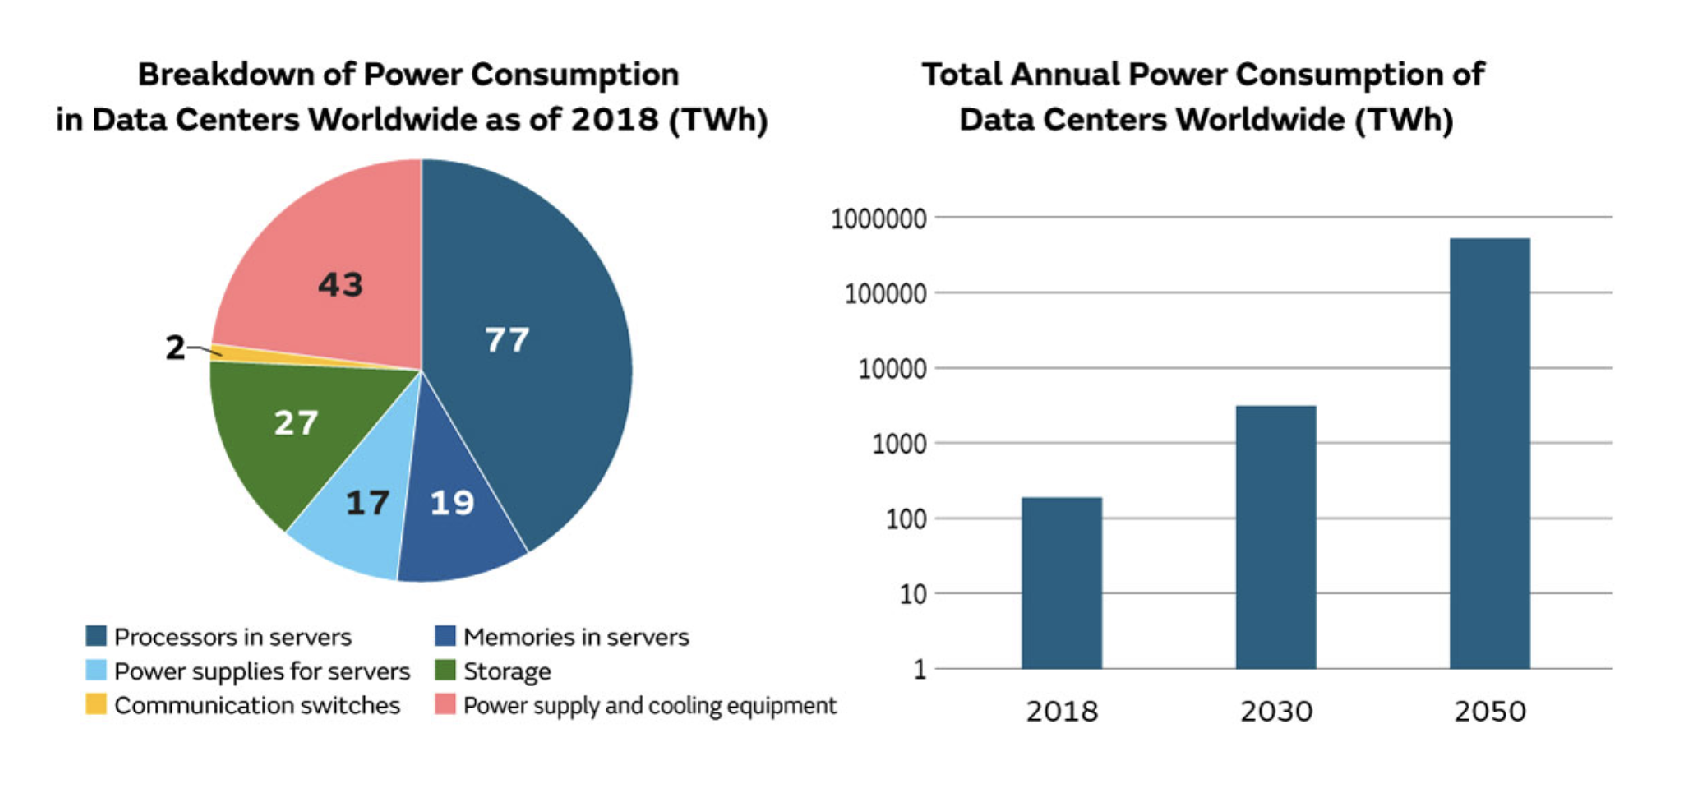
\includegraphics[scale=0.5]{fig/01/01-motivation.pdf}
    \small
    \caption{Breakdown of power consumption in data centers}
    \label{fig:01-motivation}
    \tiny
    Breakdown of power consumption in data centers and future outlook for power consumption.
\end{figure}

% Section 2: Move on to HPC and Workflows

A key driver of this trend is the exponential growth in data collection, storage, and processing across scientific disciplines. Scientific Workflow Management Systems (SWMSs) have become essential tools for managing this complexity, enabling researchers to exploit computing clusters for large-scale data analysis in domains such as remote sensing, astronomy, and bioinformatics \cite{Coleman_2021}. However, workflows executed through SWMSs are often long-running, resource-intensive, and computationally demanding, which translates into high energy consumption and substantial greenhouse gas emissions. Nevertheless, practitioners face challenges in assessing which approaches for mitigation are most applicable, effective with concerns to multiple relevant objectives \cite{thamsen2025energyawareworkflowexecutionoverview}.

Grounded in the need for optimization the central objective of this work targets at the energy-aware execution of scientific workflows. Tasks within data-driven workflows often appear in multiple instances and may vary substantially depending on input data, parameters, or execution environments in their patterns in resource demand, energy consumption, and result in fluctuating carbon emissions and runtimes rather than constant behavior. By investigating task behavior during parallel execution we address an important aspect of workflow research that has received limited attention during the last years \cite{9284517} \cite{Choudhary_2022} \cite{Durillo_2014}.
We formulate our approach by continuous monitoring to enable fine-grained, time-dependent task models that accurately capture resource usage patterns. We are specifically interested how knowledge about task behavior over time can enhance the co-location process being the intermediate stage between task-to-machine mapping and scheduling—where decisions.
Consequently, we expect that making informed decisions about which tasks share compute resources can lead to more balanced performance, improved resource utilization, and greater energy efficiency.
While related concepts have been explored in the context of co-scheduling at the operating system level or in cloud environments where batch jobs run alongside latency-critical services, the online co-location problem addressed here differs. In our setting, decisions about which tasks to execute together on the same virtual machine must be made dynamically at each scheduling interval, requiring continuous adaptation to the current workflow state and resource conditions. The importance of such decisions can be illustrated through an example by \cite{inproceedings}. Consider two compute-bound programs (A1, A2) and two memory-bound programs (B1, B2) to be co-scheduled across two nodes. If both compute-bound tasks share one node while both memory-bound tasks share the other, the memory-intensive programs will heavily compete for bandwidth, causing severe slowdowns and doubling their execution time. In contrast, pairing each compute-bound task with a memory-bound one allows both to utilize different resources efficiently, resulting in no slowdown at all. This demonstrates two fundamental principles of co-location: (i) tasks that heavily use the same resource should not be co-located, and (ii) complementary resource usage—such as pairing CPU-intensive and memory-intensive workloads—can maximize system performance.
Furthermore, previous studies have shown that effective co-scheduling of this kind can significantly enhance both energy efficiency and system throughput in high-performance computing environments. In the best cases, runtime can be reduced by up to 28\% and total energy consumption by approximately 12\% compared to isolated, dedicated execution. However, the extent of improvement depends strongly on the diversity and ratio of jobs in the scheduling queue \cite{7349920}. To address this, we propose a hierarchical clustering approach that groups tasks by dissimilarity to encourage complementary co-location. Futhermore we conduct experiments to verify the findings by \cite{inproceedings}.Lastly, our co-location mechanism is integrated into a workflow simulation framework, where several scheduling algorithms are implemented to demonstrate how informed, runtime co-location decisions can enhance task mapping and overall workflow efficiency.

% TODO: make cursive
These challenges motivate the central goal of this work: modelling the complementary co-location of scientific workflow tasks using fine-grained, time-dependent resource usage profiles and embedding it into workflow execution for energy and performance aware decision making during runtime.

\subsection{Research Question \& Core Contributions}
\label{subse:research_question_core_contributions}

The central questions this thesis seeks to address are:

\begin{enumerate}[label=\textbf{RQ}\arabic*]
    \item How can fine-grained, time-dependent models of workflow tasks be developed to capture fluctuating patterns of computational resource usage and energy consumption during execution?
    \item How can the co-location of workflow tasks be modeled so that their interference is minimized leading to lower overall energy consumption?
    \item How can energy-aware co-location models be integrated into the workflow execution phase?
\end{enumerate}

% TODO: Add footnote for nf-core repo
The resulting core contributions of this thesis are:
\begin{itemize}
    \item The implementation of a monitoring client, capable of serving the relevant monitoring layers for scientific workflow execution by collecting fine-grained, time-dependent resource usage data for workflow tasks.
    \item The design and further development of a task co-location approach that utilizes time series data to compute for any given set of tasks clusters with complementary resource usage patterns.
    \item The development of novel scheduling algorithms that integrate the proposed co-location approach into the workflow execution phase.
    \item The conceptual implementation of a scheduler, able to predict the performance and energy consumption of co-located tasks using two machine learning models.
    \item The evaluation of the co-location approach in simulation using 9 nf-core workflows, demonstrating its effectiveness in reducing energy consumption while maintaining performance.
\end{itemize}
\subsection{Structure of the Thesis}
\label{subse:structure_of_the_thesis}
The remainder of this thesis is structured as follows: Chapter \ref{cha:background} presents the fundamentals of this work, covering performance monitoring, scientific workflow systems, the co-location problem, cluster resource management and machine learning. Chapter \ref{cha:relatedwork} introduces related work within the domain of optimizing Scientifc Workflow execution and objectives in line with these of this work. Furthermore, Chapter \ref{cha:approach} depicts the approach to the problem in both a theoretical and practical manner and ultimately defines the realization of the approach. The corresponding implementation is elaborated in Chapter \ref{cha:implementation}. Moreover, Chapter \ref{cha:evaluation} evaluates the steps conducted to achieve the implementation of the overall approach using both empirical data and a simulation environment. Chapter \ref{cha:discussion} interprets the key findings and discusses some limitations of this work. Finally, Chapter 8 concludes this thesis and gives an outlook on the impact of this work for the future.
